\chapter*{Ejercicio 4}

\textbf{4.}  Diseñar un circuito decodificador con 4 entradas para la siguiente tabla de verdad, donde - denota cualquier valor, 0 o 1:

\begin{center}
        \begin{tabular}{|c c c c|c c c|}
        \hline
        \multicolumn{4}{|c|}{Entradas} &
        \multicolumn{3}{|c|}{Salidas} \\ \hline
        E1 & E2 & E3 & E4 & S1 & S2 & S3 \\ \hline
        0 & 0 & 0 & 0 & 0 & 0 & 0 \\ \hline
        0 & 0 & 0 & 1 & 0 & 0 & 1 \\ \hline
        0 & 0 & 1 & - & 0 & 1 & 1 \\ \hline
        0 & 1 & - & - & 1 & 0 & 1 \\ \hline
        1 & - & - & - & 1 & 1 & 1 \\ \hline
        \end{tabular}
        %\caption{Tabla de coches disponibles}%
        \label{tab:coches}
\end{center}

Dadas estas entradas y Salidas, diseñaremos el circuito. \\
Primero, definamos las expresiones que con estas entradas generan cada salida. \\
\begin{align*}
E_{1}+E_{2}=S_{1} \\
E_{1} + \overline{E_{2}}E_{3} = S_{2} \\
E_{1} + E_{2} + E_{3} +E_{4} = S_{3} \\
\end{align*}
Esto quiere decir que para la Salida 1 usaremos una compuerta $OR$ con $E_{1}$ y $E_{1}$, para la Salida 2 usaremos una compuerta $OR$ con $E_{1}$ y con la Salida de una entrada $AND$ de el complemento de $E_{2}$ con $E_{3}$, por último para la Salida 3 usaremos una compuerta $OR$ de todas las entradas. \\
\newline
El circuito resulta así: (Veremos también lo que resulta con las diferentes entradas.) \\
\textbf{NOTA:} Para los Entradas con guión en la Tabla este circuito va a funcionar y regresará las salidas esperadas, ya sea 0 o 1.

\begin{figure*}
    \centering
    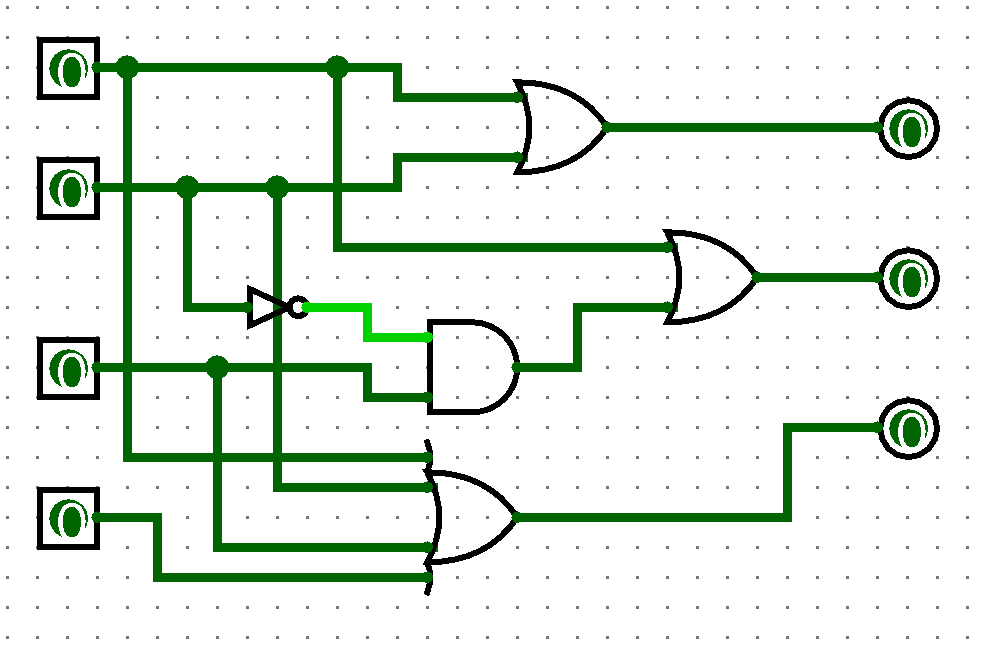
\includegraphics[height = 0.33\textheight]{recursos/Ejercicio4/CircuitoDecodificador.png}\par
    \caption*{Circuito Decodificador}
\end{figure*} 

\begin{figure*}
	\centering
    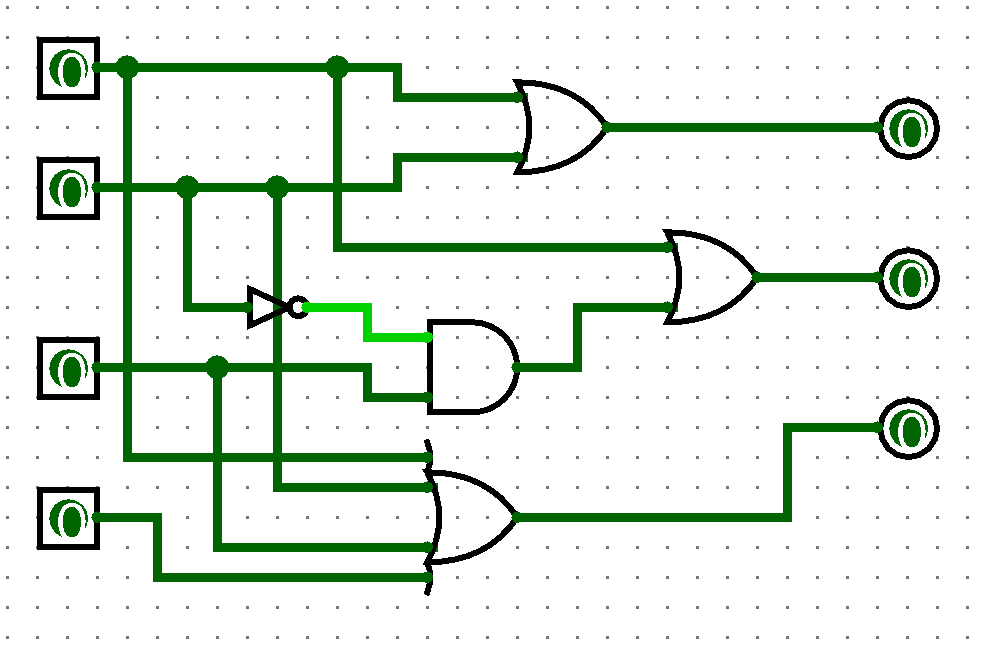
\includegraphics[height = 0.25\textheight]{recursos/Ejercicio4/1ej4.png}\par
    \caption*{Con $E_{1}=0$, $E_{2}=0$, $E_{3}=0$ y $E_{4}=0$}
    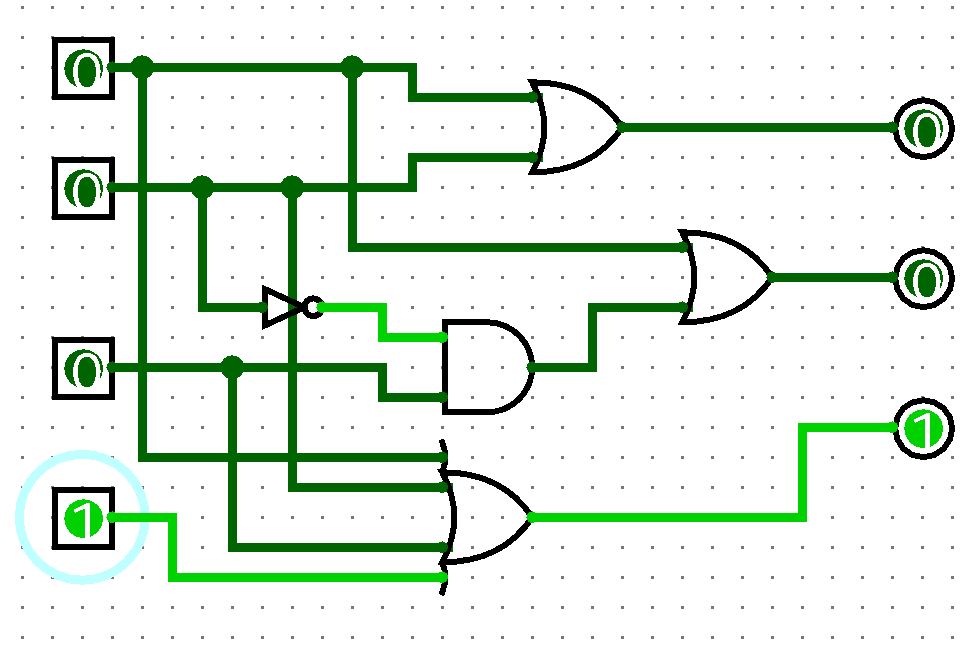
\includegraphics[height = 0.25\textheight]{recursos/Ejercicio4/2ej4.png}\par
    \caption*{Con $E_{1}=0$, $E_{2}=0$, $E_{3}=0$ y $E_{4}=1$}
    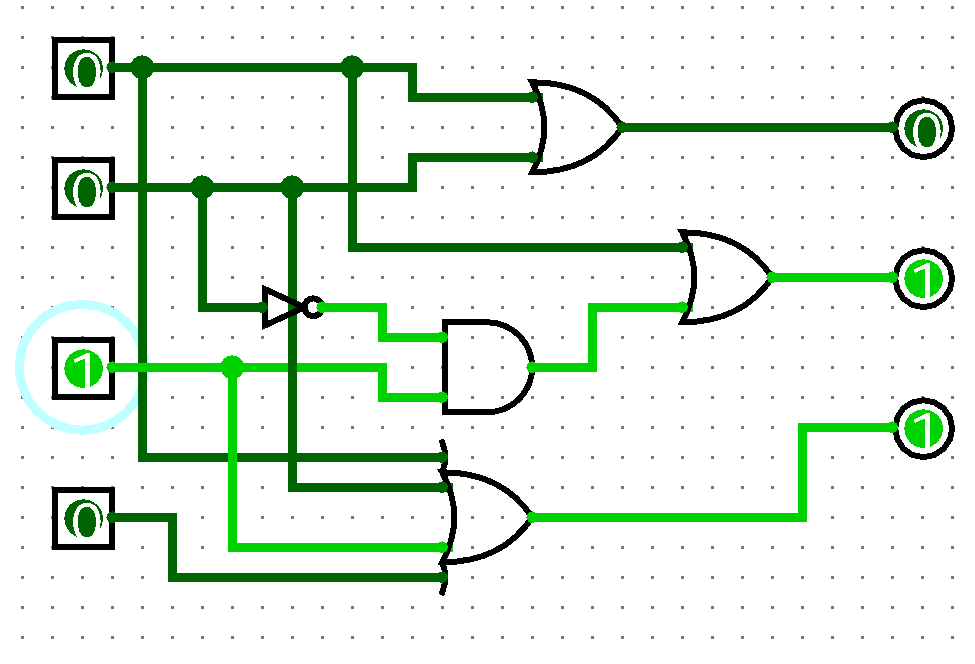
\includegraphics[height = 0.25\textheight]{recursos/Ejercicio4/3ej4.png}\par
    \caption*{Con $E_{1}=0$, $E_{2}=0$, $E_{3}=1$ y $E_{4}=0$}

\end{figure*}
\newpage
\begin{figure*}
	\centering
    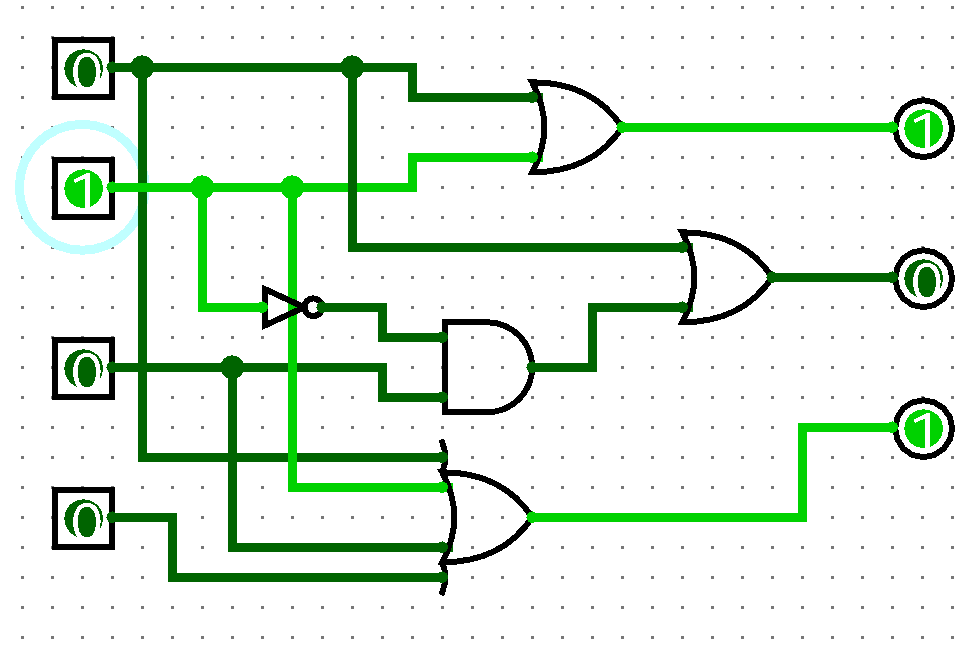
\includegraphics[height = 0.25\textheight]{recursos/Ejercicio4/4ej4.png}\par
    \caption*{Con $E_{1}=0$, $E_{2}=1$, $E_{3}=0$ y $E_{4}=0$}
    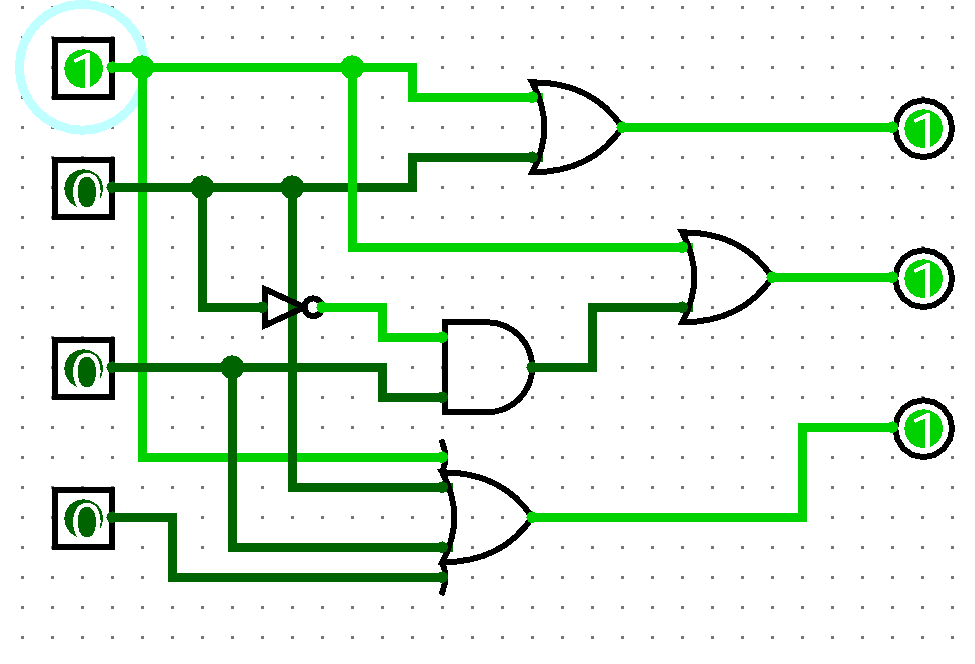
\includegraphics[height = 0.25\textheight]{recursos/Ejercicio4/5ej4.png}\par
    \caption*{Con $E_{1}=1$, $E_{2}=0$, $E_{3}=0$ y $E_{4}=0$}
\end{figure*}
%\textbf{NOTA:} Para los Entradas con guión en la Tabla este circuito va a funcionar y regresará las salidas esperadas, ya sea 0 o 1.